% ---------------------------------------------------------------------------
% Figure 4. The CVES four-layer runtime validation pipeline.
%
% VERIFIED AGAINST LIVE SOURCE, 2026-11-25:
%   * layer entry points .. engine/cves.py: l1_parse (208), l2_constitutional
%                           (318), l3_ensemble (502), l4_statistical (630).
%   * call sites .......... engine/elite_agents_v3.py: L1 at 1179, L2 at 1187
%                           (generative, with reprompt), 1218 and 1228
%                           (fallback and rule-based, logging only, NO
%                           reprompt), L3 at 1283 and L4 at 1286, both once
%                           per year over the completed set of seven.
%   * cadence ............. L1 and L2 run PER DECISION inside the seven-role
%                           loop; L3 and L4 run ONCE PER YEAR across all seven.
%                           The submitted figure drew four layers in a single
%                           flat sequence, which misstated this.
%   * L4 behaviour ........ engine/cves.py:60, L4_MODE = "flag", log the
%                           outlier and KEEP the decision. "strip" exists but
%                           is not enabled and requires an author decision.
%   * artefacts ........... per-scenario filenames (bug #18 split). The
%                           submitted manuscript named the pre-split files.
%
% NEW SINCE SUBMISSION, and drawn here because it is load bearing: the L2
% reprompt path is now schema-validated, and a malformed revision falls back
% loudly to the mechanically corrected decision (commit 6150118). Before that
% fix one malformed revision aborted an entire 50-year run.
% ---------------------------------------------------------------------------
\documentclass[border=10pt]{standalone}
% ---------------------------------------------------------------------------
% kanova-figstyle.tex
% Single source of truth for the visual style of every Ka-Nova figure.
%
% Reviewer 1, concern 6 asked that "fonts, labels, symbols, line weights, and
% overall graphical style" be made consistent across figures. Every schematic
% inputs this file and defines no local colours, line widths or fonts, so the
% consistency is structural rather than something maintained by eye.
%
% Design constraints, all deliberate:
%   * Vector output only. No raster element appears in any figure.
%   * Greyscale safe. IEEE Access prints in colour but is read in greyscale.
%     Civilian and military elements are separated by fill LIGHTNESS and by
%     border dash pattern, never by hue alone, so the distinction survives a
%     monochrome printer.
%   * Sans-serif labels at 8 pt, per the IEEE Author Center guidance for
%     figure text, applied identically in all four figures.
%   * Three line weights only, listed below. No figure introduces a fourth.
% ---------------------------------------------------------------------------

\usepackage{tikz}
\usetikzlibrary{arrows.meta,positioning,calc,fit,backgrounds,shapes.geometric,%
                decorations.pathreplacing,shapes.symbols,shapes.multipart}
\usepackage[scaled=0.92]{helvet}
\renewcommand{\familydefault}{\sfdefault}

% --- Palette. Lightness values chosen to stay distinguishable in greyscale. --
\definecolor{knink}{RGB}{26,26,26}        % all text and borders
\definecolor{knrule}{RGB}{120,120,120}    % secondary rules, annotations
\definecolor{knfillA}{RGB}{244,244,244}   % lightest  structural / container
\definecolor{knfillB}{RGB}{232,236,241}   % light     engine / mechanism
\definecolor{knfillC}{RGB}{214,222,232}   % mid       constitutional layer
\definecolor{knciv}{RGB}{226,235,228}     % civilian  chain  (lighter)
\definecolor{knmil}{RGB}{206,206,206}     % military  chain  (darker)
\definecolor{knaccent}{RGB}{140,30,30}    % CVES interception, used sparingly
\definecolor{knstore}{RGB}{250,246,235}   % persisted artefact

% --- The only three line weights used anywhere. ----------------------------
\newcommand{\knthin}{0.4pt}
\newcommand{\knnorm}{0.7pt}
\newcommand{\knbold}{1.1pt}

% --- Typography inside figures. -------------------------------------------
\newcommand{\knlabel}[1]{{\fontsize{8}{9.6}\selectfont #1}}
\newcommand{\knsmall}[1]{{\fontsize{7}{8.4}\selectfont #1}}
\newcommand{\kntiny}[1]{{\fontsize{6}{7.2}\selectfont #1}}
\newcommand{\knhead}[1]{{\fontsize{8}{9.6}\selectfont\bfseries #1}}
\newcommand{\kncode}[1]{{\fontsize{7}{8.4}\selectfont\ttfamily #1}}

\tikzset{
  every node/.style     = {font=\fontsize{8}{9.6}\selectfont, text=knink,
                           align=center, inner sep=3pt},
  % process / component box
  knbox/.style          = {draw=knink, line width=\knnorm, fill=knfillB,
                           rounded corners=1.5pt, minimum height=7mm,
                           inner xsep=4pt, inner ysep=3pt},
  % constitutional layer box
  knconst/.style        = {knbox, fill=knfillC},
  % passive container / grouping
  kngroup/.style        = {draw=knrule, line width=\knthin, fill=knfillA,
                           rounded corners=2.5pt, dash pattern=on 2pt off 1.5pt,
                           inner sep=6pt},
  % persisted artefact on disk
  knfile/.style         = {draw=knink, line width=\knnorm, fill=knstore,
                           rounded corners=0pt, minimum height=6.5mm,
                           inner xsep=4pt},
  % civilian elite role: lighter fill, solid border
  knrolec/.style        = {draw=knink, line width=\knnorm, fill=knciv,
                           rounded corners=1.5pt, minimum height=6mm,
                           minimum width=42mm, inner xsep=3pt, inner ysep=2pt},
  % military elite role: darker fill, dashed border. Two cues, not one.
  knrolem/.style        = {draw=knink, line width=\knnorm, fill=knmil,
                           rounded corners=1.5pt, dash pattern=on 3pt off 1.5pt,
                           minimum height=6mm, minimum width=42mm,
                           inner xsep=3pt, inner ysep=2pt},
  % CVES validation layer
  knlayer/.style        = {draw=knink, line width=\knnorm, fill=knfillB,
                           rounded corners=1.5pt, minimum height=8mm,
                           minimum width=30mm},
  % decision point
  kndec/.style          = {draw=knink, line width=\knnorm, fill=knfillA,
                           diamond, aspect=2.4, inner sep=1.5pt},
  % numbered step marker
  knstep/.style         = {draw=knink, line width=\knnorm, fill=white,
                           circle, inner sep=0pt, minimum size=4.6mm,
                           font=\fontsize{7}{7}\selectfont\bfseries},
  % --- edges. One arrow tip shape in the whole figure set. ----------------
  knflow/.style         = {draw=knink, line width=\knnorm,
                           -{Stealth[length=1.9mm, width=1.4mm]}},
  knflowbold/.style     = {knflow, line width=\knbold},
  knread/.style         = {draw=knrule, line width=\knthin,
                           dash pattern=on 1.5pt off 1.5pt,
                           -{Stealth[length=1.6mm, width=1.2mm]}},
  knblock/.style        = {draw=knaccent, line width=\knbold,
                           -{Bar[width=2.2mm]}},
  knnote/.style         = {font=\fontsize{6}{7.2}\selectfont, text=knrule,
                           align=left, inner sep=1.5pt},
  % panel / section heading, bold at body size
  knpanelhead/.style    = {font=\fontsize{8}{9.6}\selectfont\bfseries,
                           text=knink, align=center, inner sep=2pt},
}

\begin{document}
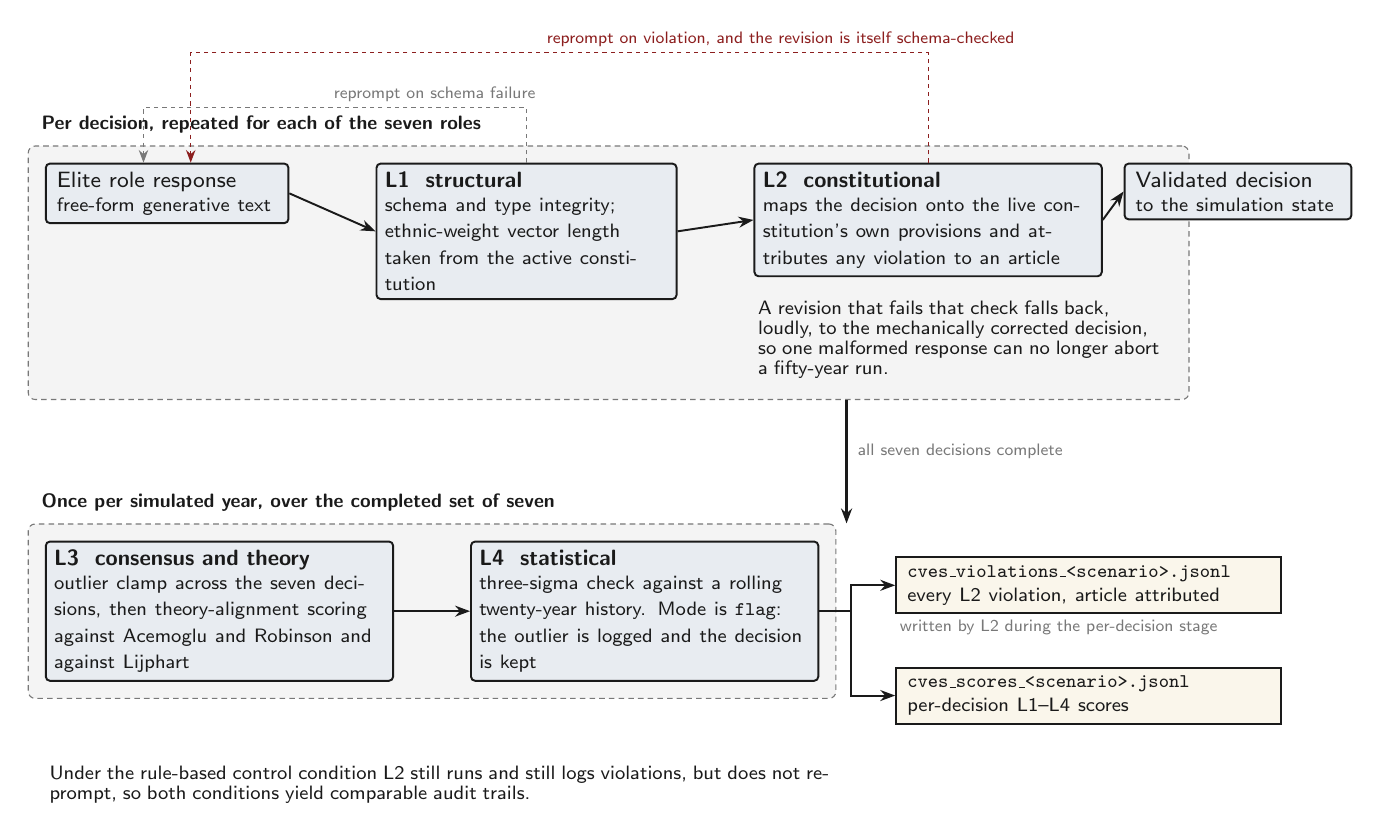
\begin{tikzpicture}[x=1mm, y=1mm]

\tikzset{
  L/.style={knlayer, align=left, minimum width=0pt, anchor=north west},
  art/.style={knfile, align=left, anchor=north west},
  B/.style={knbox, align=left, anchor=north west},
}

% ===== BAND A, per decision ===============================================
\node[B, text width=28mm] (resp) at (0,0)
  {\knlabel{Elite role response}\\[-1pt]\knsmall{free-form generative text}};

\node[L, text width=36mm] (l1) at (42,0)
  {\knhead{L1\ \ structural}\\[-1pt]\knsmall{schema and type integrity;
   ethnic-weight vector length taken from the active constitution}};

\node[L, text width=42mm] (l2) at (90,0)
  {\knhead{L2\ \ constitutional}\\[-1pt]\knsmall{maps the decision onto the live
   constitution's own provisions and attributes any violation to an article}};

\node[B, text width=26mm] (sim) at (137,0)
  {\knlabel{Validated decision}\\[-1pt]\knsmall{to the simulation state}};

\draw[knflow] (resp.east) -- (l1.west);
\draw[knflow] (l1.east)   -- (l2.west);
\draw[knflow] (l2.east)   -- (sim.west);

% reprompt arcs, stacked so they never cross
\draw[knread] (l1.north) |- ($(resp.north)+(-3,7)$)
   node[knnote, pos=0.62, anchor=south, yshift=0.4] {reprompt on schema failure}
   -- ($(resp.north)+(-3,0)$);
\draw[knread, draw=knaccent] (l2.north) |- ($(resp.north)+(3,14)$)
   node[knnote, pos=0.60, anchor=south, yshift=0.4, text=knaccent]
   {reprompt on violation, and the revision is itself schema-checked}
   -- ($(resp.north)+(3,0)$);

\node[knnote, anchor=north west, text width=52mm, text=knink] (fbnote) at (90,-17)
  {\knsmall{A revision that fails that check falls back, loudly, to the
   mechanically corrected decision, so one malformed response can no longer
   abort a fifty-year run.}};

\begin{scope}[on background layer]
  \node[kngroup, fit=(resp)(l1)(l2)(fbnote), inner sep=6pt] (perdec) {};
\end{scope}
\node[knpanelhead, anchor=south west] at ($(perdec.north west)+(1,0.8)$)
  {\knsmall{Per decision, repeated for each of the seven roles}};

% ===== BAND B, once per year ==============================================
\node[L, text width=42mm] (l3) at (0,-48)
  {\knhead{L3\ \ consensus and theory}\\[-1pt]\knsmall{outlier clamp across the
   seven decisions, then theory-alignment scoring against Acemoglu and Robinson
   and against Lijphart}};

\node[L, text width=42mm] (l4) at (54,-48)
  {\knhead{L4\ \ statistical}\\[-1pt]\knsmall{three-sigma check against a rolling
   twenty-year history. Mode is \texttt{flag}: the outlier is logged and the
   decision is kept}};

\draw[knflow] (l3.east) -- (l4.west);

\begin{scope}[on background layer]
  \node[kngroup, fit=(l3)(l4), inner sep=6pt] (peryear) {};
\end{scope}
\node[knpanelhead, anchor=south west] at ($(peryear.north west)+(1,0.8)$)
  {\knsmall{Once per simulated year, over the completed set of seven}};

% handover between the bands
\draw[knflowbold] ($(perdec.south west)+(104,0)$) -- ++(0,-6)
  node[knnote, anchor=west, xshift=2, yshift=-1.5] {all seven decisions complete}
  -- ($(peryear.north west)+(104,0)$);

% ===== artefacts ==========================================================
\node[art, text width=46mm] (viol) at (108,-50)
  {\kncode{cves\_violations\_<scenario>.jsonl}\\[-1pt]\knsmall{every L2 violation, article attributed}};
\node[art, text width=46mm] (scor) at (108,-64)
  {\kncode{cves\_scores\_<scenario>.jsonl}\\[-1pt]\knsmall{per-decision L1--L4 scores}};

\draw[knflow] (l4.east) -- ++(4,0) |- (viol.west);
\draw[knflow] (l4.east) -- ++(4,0) |- (scor.west);
% L2 writes the violation log directly during the per-decision stage; stated
% as a note rather than drawn, because the edge had to cross the whole figure.
\node[knnote, anchor=north west, text width=46mm] at (108,-57.5)
  {written by L2 during the per-decision stage};

% ===== rule-based caveat ==================================================
\node[knnote, anchor=north west, text width=100mm, text=knink] at (0,-76)
  {\knsmall{Under the rule-based control condition L2 still runs and still logs
   violations, but does not reprompt, so both conditions yield comparable audit
   trails.}};

\end{tikzpicture}
\end{document}
